% !TeX root = ../main.tex

\chapter{实验设计}

\section{系统功能性测试}
在系统进入内测阶段,我们对系统进行了功能性测试。按照需求说明书的标准,我们测
试了系统的所有功能。图~\ref{fig:test1} 是系统功能性测试用例表。用例表是测试上传表决数据的测试用例。

\begin{figure}[!htp]
    \centering
    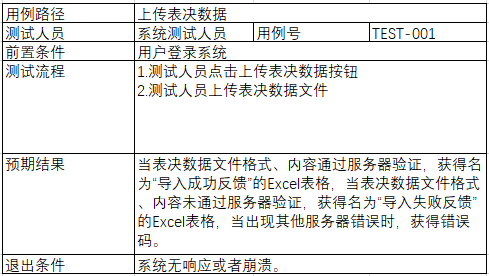
\includegraphics[height=5cm]{test1.png}
    \caption{测试用例表}
    \label{fig:test1}
  \end{figure}

  表~\ref{fig:test2}是我们进行功能性测试的结果。严重错误是指用户操作完系统无响应,系统发生了崩溃;而普通错误主要指在人机交互中的出错;而小错误则是一些显示上的字段错误或
  者页面编排上的小错误。在每次测试迭代过程中,我们都按照上一轮测试的结果不断进行
  修正,不断优化系统。

  \begin{table}[h!]
    \begin{center}
      \caption{系统功能性测试结果}
      \label{fig:test2}
      \begin{tabular}{ c c c c }
        \hline
        \textbf{测试轮数} & 1 & 2 & 3 \\
        \hline
        \textbf{小错误} & 28 & 5 & 0 \\
        \textbf{普通错误} & 20 & 2 & 0 \\
        \textbf{严重错误} & 5 & 1 & 0 \\
        \hline
      \end{tabular}
    \end{center}
  \end{table}

\section{系统性能测试}
在满足功能需求的前提下,我们需要保证系统的性能需求。本节性能测试将主要介绍三个测试,一是前端组件更新性能测试,二是 Mongo 写入性能测试,三是集群 Kafka 订阅发布性能测试。

\subsection{前端组件更新性能测试}
前端测试页面包含一个 table,通过脚本生成数据,使用 immutable.js 的 Map 存储数据,更新数据并计算平均消耗时间,测试页面如图~\ref{fig:test3}。测试页面中数据长度代表此表中将要生成的数据的数据量级别。更改数据长度后,点击生成数据可以通过编写的脚本代码在前端随机生成对应数据长度的数据并存入前端 immutable.js 的 Map 中,生成数据后点击开始更新,前端开始不间断随机更新一条 immutable.js 的 Map 中存储的数据的内容并重新渲染前端组件,在开始更新后点击报告现状,报告现状会提示当前前端组件中已经成功更新渲染的数据条数以及平均更新渲染每条数据的耗时。

\begin{figure}[!htp]
    \centering
    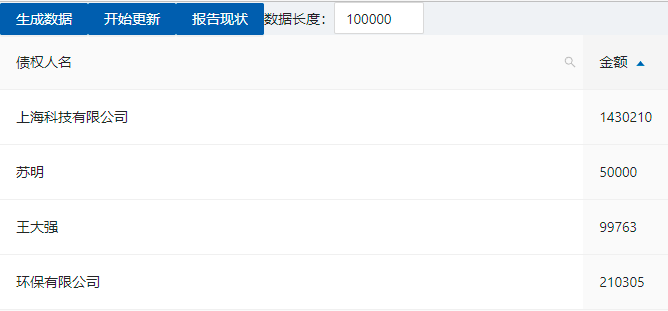
\includegraphics[height=6cm]{test3.png}
    \caption{前端测试页面}
    \label{fig:test3}
  \end{figure}

  为了测试前端在使用了 immutable.js 的 Map 进行数据存储后,在 100000 条数据的情况下平均每条数据的更新渲染所需时间,在测试页面输入数据长度为 100000,点击生成数据并点击开始更新,等待一段时间后点击报告现状,得到平均更新所需时间如如图~\ref{fig:test4},在表格 100000 条数据的情况下,平均更新每条信息所花费的时间为 0.13 ms,即在前端组件中更新 10000 条数据并渲染总共仅需 1.3 s,可以满足业务的需求。

  \begin{figure}[!htp]
    \centering
    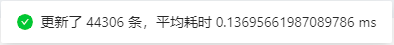
\includegraphics[height=1.5cm]{test4.png}
    \caption{前端测试结果}
    \label{fig:test4}
  \end{figure}

  \subsection{系统测试}
  \begin{figure}[!htp]
    \centering
    \begin{subfigure}{0.56\textwidth}
      \centering
      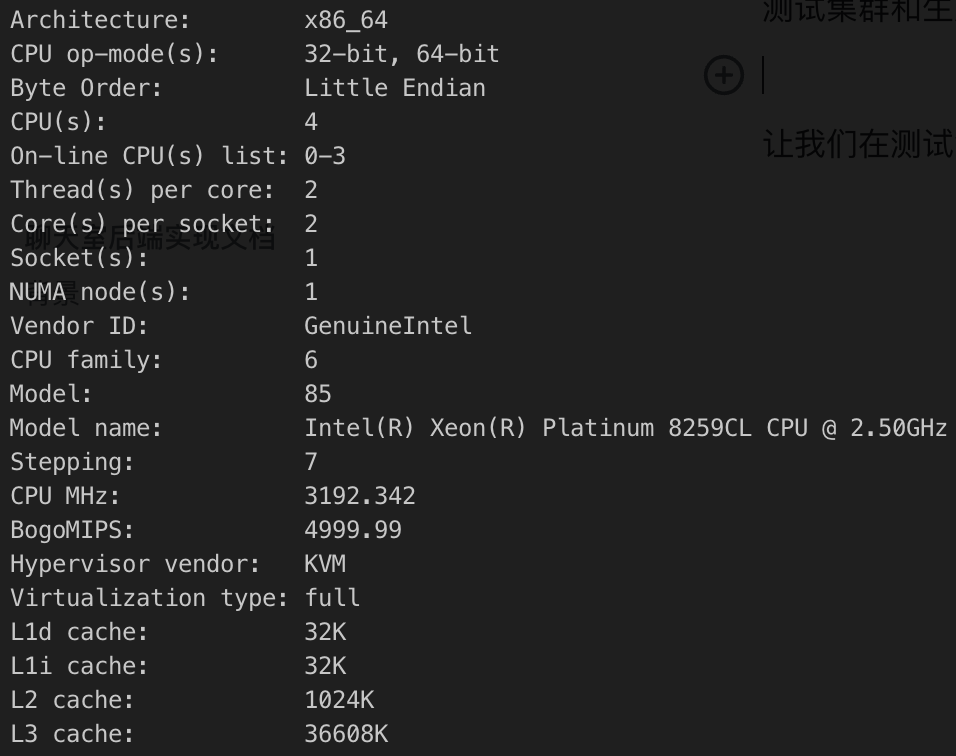
\includegraphics[height=6cm,width=8.1cm]{testEnv1.png}
      \caption{}
    \end{subfigure}
    \begin{subfigure}{0.43\textwidth}
      \centering
      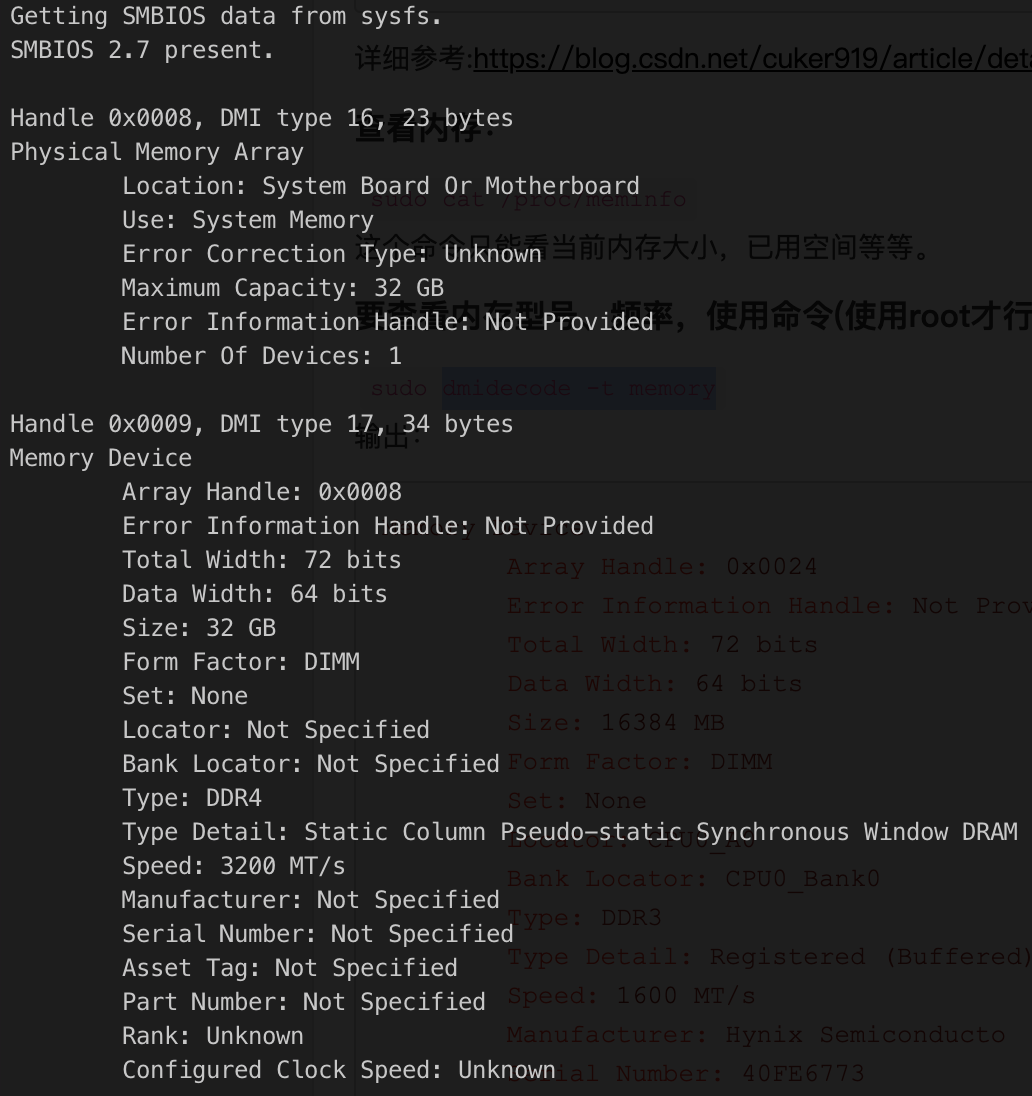
\includegraphics[height=6cm,width=5.7cm]{testEnv2.png}
      \caption{}
    \end{subfigure}
    \caption{测试环境参数}
    \label{fig:testEnv}
  \end{figure}
  进行系统测试的测试环境参数如图~\ref{fig:testEnv}所示。在此环境下测试 10 万并发量级别下从发送到实时服务到持久化到 Mongo 数据库中总的耗时。通过记录消息达到实时服务的时间,准备生产消息的时间,完成消费消息的时间,准备存入 Mongo 数据库的时间作为数据存入 Mongo 数据库中(此处不使用 Redis 集群作为缓存),成功存入后记录完成存入 Mongo 数据库的时间并记录到日志文件中。通过记录数据计算请求在本系统中平均响应时间,Kafka 平均响应时间及 Mongo 数据库平均写入时间,结果如表~\ref{fig:test7}。

  \begin{table}[h!]
    \begin{center}
      \caption{系统测试}
      \label{fig:test7}
      \begin{tabular}{ c c c c }
        \hline
        \textbf{并发量} & \textbf{平均响应时间(ms)
        } & \textbf{Kafka 平均响应时间(ms)
        } & \textbf{Mongo 平均写入耗时(ms)
        } \\
        \hline
        100000 & 4312 & 261 & 4043 \\
        \hline
      \end{tabular}
    \end{center}
  \end{table}

  根据实验结果,系统在 10 万并发量下平均一次响应所需时间为 4312 ms,其中 Kafka 的平均响应时间为 261 ms,占总时间的 6\%,Mongo 写入的平均时间为 4043 ms,占总时间的 93.8\%,明显 Mongo 的写入性能为系统的性能瓶颈,除开 Mongo 写入消耗的时间后,系统延迟并不高。

  本债权人会议系统作为高并发系统,可能存在短时间内请求过多使服务器服务宕机
的情况,可能出现高并发情况的功能有实时表决和实时聊天,如果在短时间内大量债权人同
时投票则实时表决会在短时间内出现大量请求,实时聊天同理因此增加了 Kafka 集群用作流量削峰,防止系统由于请求压力过大崩溃。通过前面的实验探知本系统的性能瓶颈为 Mongo 写入性能,下面我们对 Mongo 的本系统写入性能进行实际测试。

\begin{table}[h!]
  \begin{center}
    \caption{Mongo 写入性能测试}
    \label{fig:test5}
    \begin{tabular}{ c c c c }
      \hline
      \textbf{并发量} & \textbf{平均响应时间(ms)
      } & \textbf{P95值(ms)
      } & \textbf{P95平均值(ms)
      } \\
      \hline
      50 & 105 & 157 & 102 \\
      100 & 116 & 194 & 112 \\
      200 & 165 & 300 & 157 \\
      300 & 264 & 418 & 255 \\
      400 & 295 & 510 & 279 \\
      500 & 724 & 1007 & 702 \\
      600 & 864 & 1264 & 840 \\
      700 & 971 & 1559 & 937 \\
      800 & 1032 & 1584 & 997 \\
      900 & 1215 & 1864 & 1171 \\
      \hline
    \end{tabular}
  \end{center}
\end{table}

本文使用 Jmeter 测试工具对 Mongo 写入性能进行了测试,测试了 Mongo 集群的写入性能。创建一个测试接口,此测试接口仅含有一次写入 Mongo 操作,通过 Jmeter 测试工具提升并发量,查看平均响应时间和 P95 响应时间,表~\ref{fig:test5}是我们进行测试的结果,根据性能测试的结果,可以推算出 Mongo 仅支持 700+ QPS。

  \section{本章小结}
  本章介绍了本系统的相关实验设计。首先介绍了本系统的功能性测试,通过多轮功能性测试和优化,保证了本系统在功能性上的正确性。然后对系统性能进行了测试,确认了系统的性能瓶颈为 Mongo 写入性能,然后对本系统的 Mongo 写入性能进行了测试。